\documentclass[8pt]{article}
\usepackage{amsfonts}
\usepackage{amsmath}
\usepackage{mathtools}
\usepackage{subcaption}
\usepackage{graphicx}
\usepackage{float}
\usepackage{pythonhighlight}
\usepackage[all]{foreign}
\usepackage{hyperref}
\usepackage[capitalise]{cleveref}
\usepackage{fmtcount}
\usepackage{verbatim}
\usepackage{multicol}
\usepackage{xparse}
\usepackage{listings}
\usepackage[inline]{enumitem}
\usepackage{todonotes}

\NewDocumentCommand\weight{}{\textsf{weight}\xspace}
\DeclareMathOperator{\arctantwo}{arctan2}

\title{Fingerprint Graph Reconstruction via Probabilistic
       Logic Programming}
\author{
        Francesco Fabiano, Luca Geatti\\
        \footnotesize Department of Mathematics, Computer Science and Physics \\
        \footnotesize University of Udine\\
        \footnotesize via delle Scienze, 206, 33100 Udine, \underline{Italy}
}
\date{\footnotesize\today}


\begin{document}
\maketitle
\paragraph{Abstract}
Fingerprint recognition is a problem of fundamental importance nowadays.
Commonly, fingerprints are represented in databases as a set of
\emph{minutiae}, \ie points in the 2D space of an image with a direction and
a type attached. A fundamental problem is to reconstruct from this set of
points a graph representing the original fingerprint.  Probabilistic Logic Programming (PLP, for short)
reveals itself as a powerful framework to reason about domains characterized
by uncertainty. Among the main techniques, LPADs
perhaps are the most general, allowing one to annotate each atom in the head of
a rule with probability.  In this paper, we give an encoding of the
fingerprint graph reconstruction using PLP; in particular, we give a set of
rules which define the probability of existence of an edge and a set of
structure constraints to forbid graph structures that are not possible.
Notably, the probability attached
to each rule is not fixed \apriori: instead, the rules are
parametric, that is their probabilities are real-values variables. This allowed
us to model with greater precision the we are considering.  In the end we
propose an iterative algorithm to compute effectively the fingerprint graph from 
the minutiae information.\\~\\
\emph{This is a report for the PhD course exam on Probabilistic Logic Programming, 
held at University of Udine in the academic year 2018-2019 by Elena Bellodi.}




\section{Introduction}
Modern \textit{biometrics}-based tools exploit the fact that biometric
characteristics, used for the verification of an individual’s identity, are
unique from person to person\cite{maltoni2009handbook}.  This is why the
majority of the studies in this
field aim to generate biometric tools that are able to distinguish even twins
\cite{jain2001twin,jain2002similarity}.
%
The purpose of the above-mentioned studies is to identify the uniqueness of each
\textit{fingerprint}, facial feature or any others biometric characteristics of
a person. Fingerprints in particular play a central role, as they are
 the most used biometric characteristics. A fingerprint's image is not
stored in the database, commonly due to space issues; instead, only a set of
point of the original image, called \emph{minutiae}, is stored.
\todo[inline]{from here}
In this paper, we focus on fingerprint recognition, that is the problem of
checking whether two fingerprints images really represent the same fingerprint.
%
Among the main techniques, a particularly interesting one creates a graph from
the set of minutiae and then uses \emph{graph matching} to check the equality
of two fingerprints \cite{isenor1986fingerprint}. Therefore, a key problem is
to reconstruct from a set of minutiae the most likely graph, which is the main
problem we tackle in this paper. We refer to this as the \emph{fingerprint
graph reconstruction problem}.
\todo[inline]{to here}
Probabilistic Logic Programming (PLP, for short) reveals itself as a powerful
framework to reason about uncertain systems. It inherits from Logic Programming
the ability to write succinct yet meaningful programs, powerful inference
tools like unification, and ,from Probability Theory, the ability to reason
with uncertainty.
Among the main techniques proposed for PLP, Logic Programs with Annotated
Disjunctions (LPADs, for short) received a lot of attention, thanks to the
easiness they allow to write probabilistic logic programs; in fact, for one to
write a logic program in LPAD, it suffices to attach probability values to
the atom in the head of the rule.

In this paper, we give an LPADs-based encoding of the fingerprint graph
reconstruction problem; in particular, along with structure constraints that
forbid wrong graphs, we have rules to infer the existence of an edge with
a given probability. Notably, the probabilistic rules do \emph{not} have
a fixed probability attached: instead, we used real-valued variables to model
a probability function. The rationale behind this choice is that the
probability of existence of an edge between two minutiae is really a function
that depends, for example, on the \emph{distance} or \emph{orientation} of the minutiae themselves.
As we
will see, this allowed us to model the problem with greater precision.
Finally, we propose an algorithm that iteratively makes a query to our LPADs
program and it terminates with the reconstructed graph. 



\section{Background}
\label{sec:background}
In this section, we give some background definitions about fingerprint
recognition and probabilistic logic programming, in particular about LPADs.

\subsection{Minutiae and Fingerprint graph}
\label{sub:backfinger}
We refer to \cite{maltoni2009handbook} for the main definitions about
fingerprint recognition.  Each \emph{minutia} is an informative point of the
fingerprint, in the sense that it represents distinct features of the latter.
It can be of two type: \emph{ending}, \ie it represents one end of a ridge, or
\emph{bifurcation}, representing a point where a ridge splits into two other
ridges.  Furthermore, each minutia has attached a position in the image (\ie
coordinates along the X and Y axis) and a direction (usually expressed in
radians), representing 
\begin{enumerate*}[label=\roman*)]
  \item the direction of the corresponing ridge, in the case of an ending
        minutia;
  \item the direction of the bifurcation, in the case of a bifurcation minutia.
\end{enumerate*}
In \cref{fig:skemin}, ending minutiae are surrounded by blue circles, while
bifurcation minutiae by green one. Moreover, the short straight line exiting
outgoing of a circle represents the direction of the minutia. 

Along with the set of minutiae, usually the database contains also the
\emph{type} of the whole fingerprint: in \cref{fig:patterns}, four
types of fingerprints are pictured, \ie the ones we have considered in our study. This information is particularly important
in the context of recognition, since it represents useful background
information.  For example, to determine the probability that two
minutiae are linked is possible to check the fingerprint type and
the position of the two minutiae to give a more accurate answer
compared to the one that would be given only knowing the position of the minutiae.
Therefore, in our encoding, we will exploits both the minutiae information and
the fingerprint type. 
    
    \begin{figure}
		\centering
		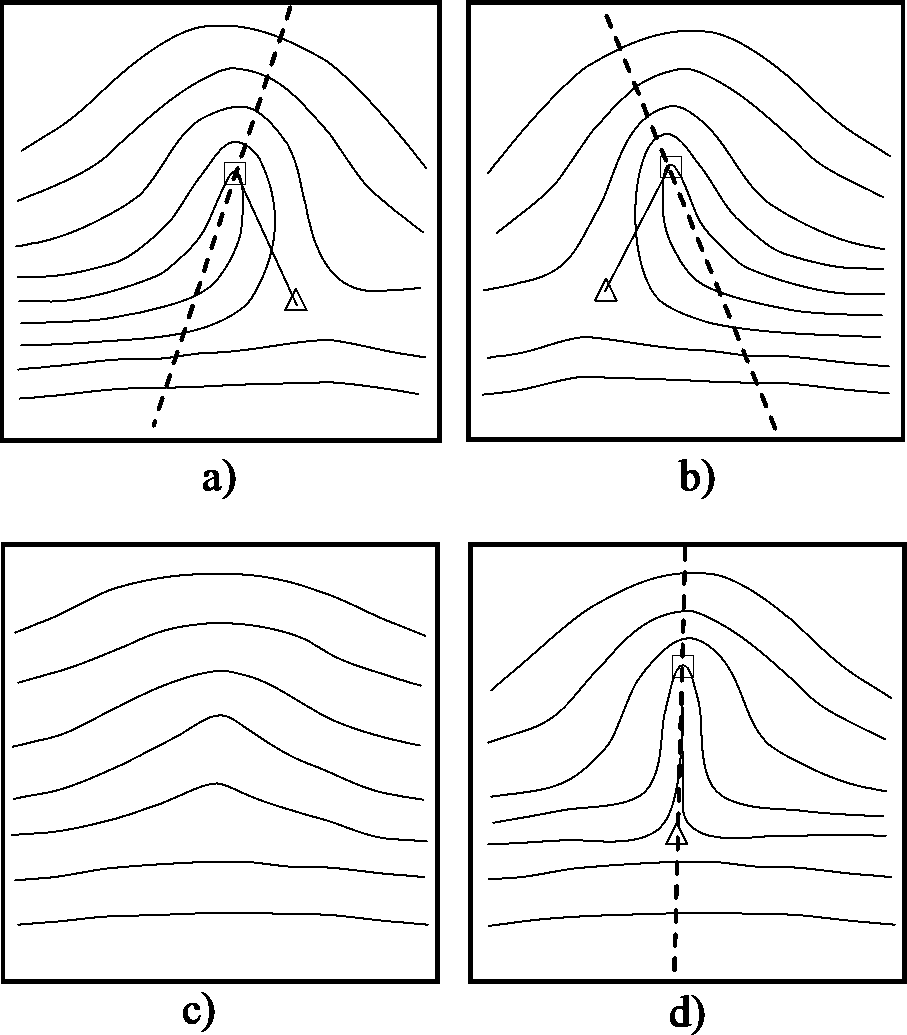
\includegraphics[scale=0.3]{img/patterns}
		\caption{Fingerprint patterns as they appear at a coarse level: 
        a) \textit{left loop}, 
        b) \textit{right loop}, 
        c) \textit{\textit{arch}}, and 
        d) tented arch; squares denote loop-type singular points, and triangles
			     delta-type singular points.}
		\label{fig:patterns}
	\end{figure}%
   
\begin{figure}
	\centering
	\begin{subfigure}{.48\textwidth}
	\centering
	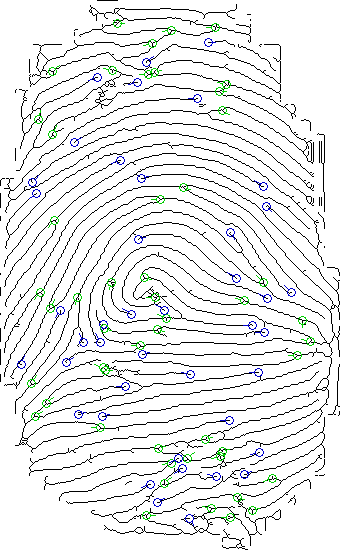
\includegraphics[width=.75\linewidth]{img/skemin}
	\caption{The skeleton and the minutiae of a fingerprint.}
	\label{fig:skemin}
	\end{subfigure}%
	\hfill
	\begin{subfigure}{.48\textwidth}
	  \centering
	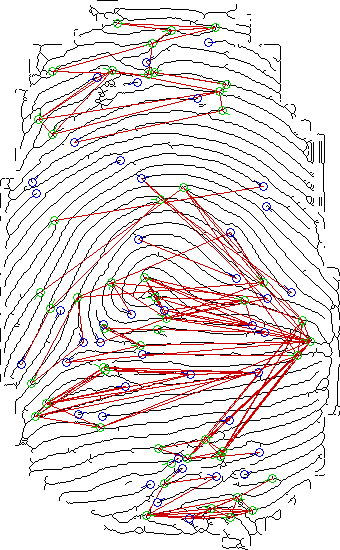
\includegraphics[width=.75\linewidth]{img/skemingraph}
	\caption{The ideal graph of the fingerprint in \cref{fig:skemin}}
	\label{fig:skemingraph}
	\end{subfigure}%
\end{figure}

The graph we want to reconstruct is a particular type of directed
\textit{graph} subjected to several structure constraints on the edges; \eg each
node can have at most one \textit{incoming edge} and at most two
\textit{outgoing}.  We refer to this as the \emph{fingerprint graph}.  The main
idea behind this graph (shown in \cref{fig:skemingraph}) is that it should
\textquoteleft emulate' the \textit{skeleton} (the black lines of
\cref{fig:skemin}) of the fingerprint.  As reconstructing this graph could be
somewhat trivial when in possession of the fingerprint's original image, it is not
when the only available information are the fingerprint's minutiae.
Unfortunately this is the case in most of the official databases where, due to
space optimization, the fingerprints are only stored as a set of minutiae along
with few other information.
    



\subsection{Logic Programs with Annotated Disjunctions}
\label{sub:lpads}
Probabilistic Logic Programming reveals itself as a powerful framework that
combines the succincteness and powerful inference aspects of logic programming
with the ability to reason with uncertainy typical of probability theory.
A fundamental approach is the one Distribution Semantics
\cite{sato1995statistical}, which defines a probability distributions over
normal logic programs, called \emph{instances}. Furthemore, this distributions
conservatively translates into probability distributions over the Herbrand's
models of the cosidered program.

Logic Programs with Annoted Disjunctions \cite{vennekens2004logic} are an
example of languages following distribution semantics. They allow the user to
annotate the atom in the head of a rule with probabilities. An LPADs consists
of a finite set of annotated disjunctive clauses $C_i$ of the form:
  \begin{align*}
    h_{i1}:\Pi_{i1}; \dots ; h_{in_i}:\Pi_{in_i} \colon- b_{i1},\dots,b_{im_i}.
  \end{align*}
where $b_{i1},\dots,b_{im_i}$ are literals, $h_{i1},\dots,h_{in_i}$ are atoms
and $\Pi_{i1},\dots,\Pi_{in_i}$ are real numbers in the interval $[0,1]$ such
that $\sum_{k=1}^{n_i} \Pi_{ik} \le 1$. Note that if $n_i=1$ and $\Pi_{i1}=1$
then $C_i$ is an Horn clause.
If $\sum_{k=1}^{n_i} \Pi_{ik} < 1$, then we are implicity assuming that there
exists an extra atom \emph{null} with attached probability $1-\sum_{k=1}^{n_i}
\Pi_{ik}$. We denote with $ground(T)$ the grounding of LPAD $T$.

In the next section, we will see how we can use LPADs to reconstruct the
fingerprint graph; in particular, given an LPAD program we will make a query
over it to infer both its truth and its probability.  As we will see, we will
exploit informations like the type of the whole fingerprint (see
\cref{fig:patterns}), the distance of two minutiae and direction of a minutiae
and so on and so forth. We will see that an accurate encoding results from the
combined use of all these considerations.







%%%%%%%%%%%%%%%%%%%%%%%%%%%%%%%%%%%%%%%%%%%%%%%%%%%%%%%
%%% Encoding
%%%%%%%%%%%%%%%%%%%%%%%%%%%%%%%%%%%%%%%%%%%%%%%%%%%%%%%
\section{Logical Encoding}
\label{sec:logicalencoding}
We start by describing the basic predicates to model the problem. In order to
model a minutia, we introduce the predicate
  \begin{center}
    \textsf{minutia(X,Y,D,T)}
  \end{center}
where $\textsf{X},\textsf{Y} \in \mathbb{N}$ are the coordinates\footnote{Note 
that the pixel with coordinates $(0,0)$ is the top left one.}
of the minutiae inside the image along the X-axis and Y-axis, respectively;
$\textsf{D} \in [0,2\pi]$ is the direction, expressed in radians; 
and $T \in \{e,b\}$ is the type of the fingerprint ($e$ stands for
\emph{ending}, $b$ for \emph{bifurcation}, see \cref{sub:backfinger}).
The second predicate is
  \begin{center}
    \textsf{type\_fingerprint(T)}
  \end{center}
where $\textsf{T}\in\{
  \textsf{tented\_archs},
  \textsf{plain\_archs},
  \textsf{left\_loop},
  \textsf{right\_loop}
\}$; 
basically, it expresses which type the overall fingerprint belongs to (see
\cref{fig:patterns}).  Finally, \textsf{max\_X(N)} and \textsf{max\_Y(N)}
express the number of pixels of the image along the X-axis and the Y-axis,
respectively.  The \emph{knowledge base} of our program is a set of ground
facts, more specifically: a set of \textsf{minutia/4} facts, one single
\textsf{type\_fingerprint/1} fact, one \textsf{max\_X/1} and one
\textsf{max\_Y/1} fact. For example:
  \begin{center}
  \begin{lstlisting}[language=Prolog,frame = single,basicstyle=\footnotesize\ttfamily]
max_Y(450).
max_X(338).
type_fingerprint(tented_archs).
minutia(338,84,3.14888994760949725,e).
minutia(47,450,0.1334635904729058,e).
minutia(39,302,0.8478169733934057,e).
...
minutia(58,256,5.31793364398966,b).
minutia(94,104,0.09966865249116204,b).
minutia(62,272,5.135242906517631,b).
  \end{lstlisting}
  \end{center}
Since the set of minutiae are normally represented in the database in XML
format, we wrote script to translate from XML to Prolog-like format.

Since what we want to infer are the existence of the edges between the minutiae
along with their probability of existence, we introduce the predicate
  \begin{center}
    \textsf{edge($X_1,Y_1,X_2,Y_2$)}
  \end{center}
where $(X_1,Y_1)$ are the coordinates of one minutia and $(X_2,Y_2)$ the
coordinate of the other minutia.
Since in our setting we want undirected edges (their direction does not
matter), some simmetry breaking constraints can be added to the encoding,
aiming at removing specular but equivalent solutions; in particular, we
constrained that there must exist only left-to-right edges with the following
constraint, which we will use as a precondition for (\ie appearing in the body
of) every rule to infer an edge:
  \begin{center}
  \begin{lstlisting}[language=Prolog,frame = single,basicstyle=\footnotesize\ttfamily]
good_edge(X1,Y1,X2,Y2) :-
   minutia(X1,Y1,_,_),
   minutia(X2,Y2,_,_),
   X1<X2.
good_edge(X1,Y1,X2,Y2) :-
   minutia(X1,Y1,_,_),
   minutia(X2,Y2,_,_),
   X1=X2,Y1<Y2. 
  \end{lstlisting}
  \end{center}





\subsection{Structure constraints}\label{sub:structure_cons}
We introduce two structure constraints to forbid wrong edges
in the final solution.
\begin{itemize}
  \item
    each B-minutia has exactly $3$ incident edges. This has been achieved
    using the \texttt{aggregate\_all} predicate, as follows:
      \begin{lstlisting}[language=Prolog,frame = single,basicstyle=\footnotesize\ttfamily]
b_inc_edge :-  aggregate_all(count, edge(X,Y,X1,Y1), Count1),
               aggregate_all(count, edge(X2,Y2,X,Y), Count2),
               Sum is Count1+Count2, Sum == 3,
               minutia(X,Y,_,b),
               minutia(X1,Y1,_,_),
               minutia(X2,Y2,_,_).
      \end{lstlisting}
  \item
    similarly, each E-minutia has exactly $2$ incident edges.
\end{itemize}
With the rules 
  \begin{lstlisting}[language=Prolog,frame = single,basicstyle=\footnotesize\ttfamily]
    valid_graph :- b_inc_edge, e_inc_edge.
    valid_graph.
  \end{lstlisting}
we impose these two structure constraints.














\section{Probabilistic Encoding}
\label{sec:probenc}
In this section, we will give the probabilistic rule to infer the existence of
an edge along with its probability. The rules are divided depending by which
type of fingerprint (see \cref{fig:patterns}) they refer to; we describe first
the rules for \emph{tented} and \emph{plain archs}, since the cases for the
remaining type will reuse these rules.

One important thing to note is that the probabilistic rule we are going to
describe have \emph{not} a fixed probability attached to the atoms in the head
of the rules. Instead, we attache real-valued variables: this allows us to give
different probability values to an atom depending by how the \emph{unification}
process occurs. By the modelling side, this permits a greater precision and
flexibility: instead of having a fixed probability and being tailored for only
one particular database of fingerprints' images, our rules are independent from
the particular test set used and do \emph{not} require the user to manually fix
the probabilities.



\subsection{Tented and Plain Archs}
Here we describe probability rules for the tented and plain archs fingerprints:
you can refer to \cref{fig:arch} as an example.

\paragraph{Direction Constraint}
In this paragraph, we give a constraint for the edges inside a tented or plain
arch fingerprint that link the \emph{direction} of the two minutiae with the
probability of existence of an edge between them.  Given two minutiae $M_1$ and
$M_2$ (of any kind) belonging to a tented or plain arch fingerprint, we note
that the probability of existence of an edge between these two respects this
rule: the more the directions of both the minutiae is close to the straight
line connecting $M_1$ and $M_2$ the more the probability is high.  For example,
in \cref{fig:arch} at the two extremes of the red line there are (at least) two
minutiae such that their direction if very close to the straight line
connecting them.  Let $M_1=(X_1,Y_1,D_1,\_)$ and $M_2=(X_2,Y_2,D_2,\_)$ be two
minutiae.  Let $\alpha_1=\arctantwo(Y1-Y2,X1-X2)$ and
$\alpha_2=\arctantwo(Y2-Y1,X2-X1)$: $\alpha_1$ (resp. $\alpha_2$) measures the
value of the angle (in randians) between the direction of $M_1$ (resp. $M_2$)
and the straight line between $M_1$ and $M_2$.  We define\footnote{Note that we
divide by $2\pi$ in order to normalize the value on the numerator and to make
it a correct probability value.}:
  \begin{align}\label{eq:distcons}
    \weight_{DIS} \coloneqq
    W \cdot (1-\frac{\lvert D1-\alpha_1\rvert+\lvert D2-\alpha_2\rvert}{2\pi})
  \end{align}
where in the case of tented archs $W=1$; in the following we will explain the
meaning of variable $W$: intuitively $W$ will represent the importance of this
rule for the fingerprint type under consideration; since we are dealing with
tented and plain archs and we want this rule to be important as the other ones,
we give it importance $W=1$. With this Distance Constraint, we give the value
$weight_{DIS}(M_1,M_2)$ to the probability of existence of an edge between
$M_1$ and $M_2$. Overall, we obtain the following LPAD's rule:
  \begin{lstlisting}[language=Prolog,frame = single,basicstyle=\footnotesize\ttfamily]
edge(X1,Y1,X2,Y2): Weight :-
                 minutia(X1,Y1,D1,_),
                 minutia(X2,Y2,D2,_),
                 good_edge(X1,Y1,X2,Y2),
                 Alpha1 is float(atan2(Y1-Y2,X1-X2)),
                 Alpha2 is float(atan2(Y2-Y1,X2-X1)),
                 Diff1 is float(abs(D1-Alpha1)),
                 Diff2 is float(abs(D2-Alpha2)),
                 weight_rule(W,Y1,Y2),
                 Weight is float(W*(1 -rdiv((Diff1+Diff2),(2*pi)))). 
  \end{lstlisting}
where the last line computes exactly \cref{eq:distcons}. In the following, when
writing the formula for a particular \texttt{weight}, we always assume that the
corresponding variable $Weight$ is attached to the atom \texttt{edge} in the
head of the rule.



\paragraph{Distance Constraints}
Here we give a total of three constraints for edges inside
a tented or plain archs fingerprint that take into consideration the
\emph{distance} between two minutiae.
Let $M_1=(X_1,Y_1,D_1,\_)$ and $M_2=(X_2,Y_2,D_2,\_)$ be two minutiae.
  \begin{itemize}
    \item \textbf{DIST\_ARCH\_1}: the more the position of $M_1$ and $M_2$
          on the Y-axis is similar, the more an edge between $M_1$ and $M_2$
          is likely to exist. We assign $\weight_{DA1}$ to the probability
          of existence of this edge, where:
            \begin{align*}
              \weight_{DA1} \coloneqq 1-\frac{\lvert Y1-Y2\rvert}{max\_Y}
            \end{align*}
          Note that the division by $max\_Y$ is necessary in order to
          normalize the value $\lvert Y1-Y2\rvert$ and make it a correct
          probability value. Intuitively, this rule says that the more two
          minutiae have the same height inside the image, the more an edge
          connecting them is likely to exist.
    \item \textbf{DIST\_ARCH\_2}: the same as the previous point, but with
          the X-axis;
    \item \textbf{DIST\_ARCH\_3}: the more the X-coordinate of the midpoint of 
          the line between $M_1$ and $M_2$ is close to the half of the image,
          the more this edge is likely to exist. In other words, we want that
          minutiae that are \emph{not balanced} w.r.t. to the center of the
          image (\eg one minuties close to the center but the other on the 
          extreme right) are unlikely. We assign $\weight_{DA3}$ to the 
          probability of existence of this edge, where:
            \begin{align*}
              \weight_{DA3} \coloneqq 1 -
              \frac{\lvert \frac{\lvert X1-X2 \rvert}{2} - \frac{max\_X}{2}
              \rvert}{max\_X}
            \end{align*}
          where $\frac{\lvert X1-X2 \rvert}{2}$ is the X-coordinate of the
          midpoint of the line between $M_1$ and $M_2$ and $\frac{max\_X}{2}$
          is the midpoint of the image; again, we normalize with the division
          by $max\_X$. Therefore, the more the difference on the numerator is
          low, the more the resulting probability is high.
  \end{itemize}






\subsection{Left and Right Loop}
In this part, we describe the probability rules for the left and right loop
fingerprints.  Since, in their upper region, left and right loop fingerprints
exhibit a behavior similar to that of tented and plain archs fingerprints (see
\cref{fig:loop} for an example), we decided to use the contraints we described
above in these cases as well. In particular, we note that in the upper region,
the behavior of a left or right fingerprint is very similar to that of a plain
of tented arch. For this reason, we parameterized \emph{Distance Constraint}
with the variable $W$:
  \begin{itemize}
    \item
      if we have a tented or plain archs fingerprint, then $W$ is $1$, meaning
      that the rule has the same weight (or \emph{importance}) for all the
      points in the image;
    \item
      otherwise, in the case of left or right loop fingerprint, $W$ is
      computed by the predicate $weight\_rule(W,Y1,Y2)$, which assigns 
      $W$ the value:
        \begin{align*}
          W \coloneqq 
          \Big\lvert 1-\frac{Y1}{max_Y} \Big\rvert 
          \cdot 
          \Big\lvert 1-\frac{Y2}{max_Y} \Big\rvert
        \end{align*}
      Therefore, the closer the two points are to the upper region of a left or
      right loop fingerprint, the more the value of $W$ is high and in turn the
      more we give weight to \emph{Distance Constraint}.
  \end{itemize}


In the following, we give probabilistic rules tailores for left-loop and
right-loop typed fingerprints.
\paragraph{Constraint LOOP}
Given a left or right loop fingerprint, we noted that the ending-type
minutiae located in the \emph{lower region} of the image are clustered along
a vertical line as shown in \cref{fig:loop}.
This behavior is captured by \emph{Constraint LOOP}, which gives to
the edge between two minutiae $M_1$ and $M_2$ belonging to a left or right loop
the probability $\weight_{LOOP}$, where:
  \begin{align*}
    \weight_{LOOP} \coloneqq
    (1-W)\cdot 
    (1-\frac{\lvert X1-X2 \rvert}{max\_X})
  \end{align*}
In words, the more $\lvert X1-X2 \rvert$ is low, the more the two points
``form" a vertical line and in turn the more $(1-\frac{\lvert X1-X2
\rvert}{max\_X})$ is high.  Again, $(1-W)$ models the fact that the more the
two minutiae are lower in the image, the more weight we want to give to the
rule.  



\paragraph{Constraints LL and LR}
Along the above-mentioned line on which the minutiae of a left or right loop
fingerprint are located, we identified another two constraints, that we call
\texttt{LL} (short for \texttt{L}eft \texttt{L}oop) and \texttt{RL} (short for
\texttt{R}ight \texttt{L}oop): minutiae have to be \emph{balanced} along the
vertical line of \cref{fig:loop}, in a very similar way we did for
\emph{DIST\_ARCH\_3}. In other words, the more the midpoint of the straight line between
two minutiae is closer to the \emph{third quartile}\footnote{For third
quartile, we wean the set of points $(X,Y)$ such that $Y=\frac{3}{4}\cdot
max\_Y$} (the lowest dotted line in \cref{fig:loop}) of the image, the more an edge between them is likely.

Overall, the probability given by \emph{Constraint LL} to the existence of an
edge is $\weight_{LL}$, where:
  \begin{itemize}
    \item
      $\weight_{LL}^\prime \coloneqq 
        (1-W) \cdot (1-\frac{X1}{max\_X}) \cdot (1-\frac{X2}{max\_X})$ 
    \item
      $\weight_{LL} \coloneqq
        \weight_{LL}^\prime \cdot (1-
        \frac{\lvert \frac{\lvert Y1-Y2 \rvert}{2} - \frac{3}{4}\cdot max\_Y
        \rvert}{max\_Y})$
  \end{itemize}
Recall that the more $(1-W)$ is high, the more we are in the lower region of
the image. In the same way, the more $\weight_{LL}^\prime$ is high, the more we
are in the bottom left region of the image.  To sum up, with $\weight_{LL}$ we
are saying that the more the points are \emph{balanced} w.r.t. the third
quartile, the more an edge between them is likely to exist.

\emph{Constrain RL} does the same except that $\weight_{RL}^\prime$ is
defined as follows:
  \begin{align*}
    \weight_{RL}^\prime \coloneqq 
      (1-W)\cdot \frac{X1}{max\_X} \cdot \frac{X2}{max\_X}
  \end{align*}
in order to give more weight to the points in the bottom right region.
\begin{figure}
	\centering
   	\begin{subfigure}{.48\textwidth}
   			\centering
	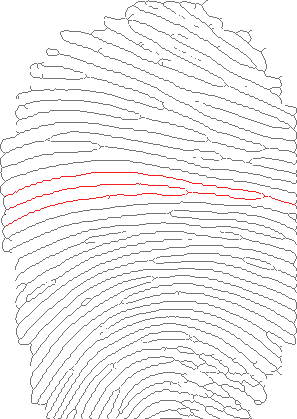
\includegraphics[width=0.9\linewidth]{img/arch}
	\caption{Skeleton of an \textit{arch} type. In red are highlighted examples of the describe ridges.}
	\label{fig:arch}
\end{subfigure}%
\hfill
\begin{subfigure}{.48\textwidth}
	\centering
	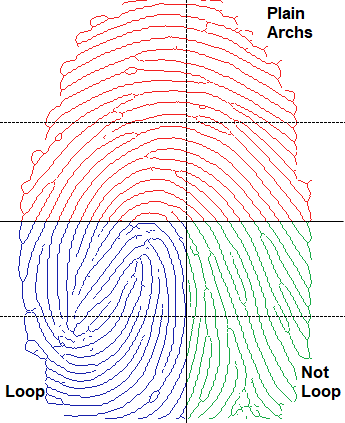
\includegraphics[width=1\linewidth]{img/loop_mod2}
	\caption{Skeleton of a \textit{left-loop} type. In blue the quadrant that encapsulates the loop while in red and green the parts captured by the arch constraints.}
	\label{fig:loop}
\end{subfigure}%
\caption{Example of the properties captured by our constraints.}
\label{fig:example}
\end{figure}











%%%%%%%%%%%%%%%%%%%%%%%%%%%%%%%%%%%%%%%%%%%%%%%%%%%%%%%%%%%%%%%
%%% GENERATION OF THE FINGERPRINT GRAPH
%%%%%%%%%%%%%%%%%%%%%%%%%%%%%%%%%%%%%%%%%%%%%%%%%%%%%%%%%%%%%%%
\section{Generation of the fingerprint graph}
\label{sec:graphgen}
We used \texttt{cplint} \cite{alberti2017cplint} both as the editor with which
to write the LPAD and as the main engine to solve all the queries that we are
going to describe \footnote{You can find the implementation of the encoding at
\url{https://github.com/lucageatti/PLP-fingerprints} or inside the
\texttt{fingerprints.pl} script under the \texttt{code} folder of this
package.}.  With the query 
  \begin{center}
  \begin{lstlisting}[language=Prolog,frame = single,basicstyle=\footnotesize\ttfamily]
findall([X1,Y1,X2,Y2,P],prob(edge(X1,Y1,X2,Y2),P),Results).
  \end{lstlisting}
  \end{center}
we can retrieve all the results of the unification of \texttt{edge(X1,Y1,X2,Y2)}
with the logic program's rules. The result is a list of this type:
  \begin{center}
  \begin{lstlisting}[language=Prolog,frame = single,basicstyle=\footnotesize\ttfamily]
Results = [
  [39, 302, 58, 256, 0.8761637920914388],
  [39, 302, 338, 84, 0.9757900620331998],
  [39, 302, 62, 272, 0.921175664640193],
  [39, 302, 47, 450, 0.901470217393874],
  ...
  [47, 450, 338, 84, 0.9445871662832741],
  [94, 104, 338, 84, 0.9562089492578153]
]
  \end{lstlisting}
  \end{center}
Each tuple in the list is an edge labeled with its probability of existence,
based on the rules we described above. This is \emph{not} the final graph
we want to retrieve, since it is just the collection of all the results
of the unification. Thus, we propose the following procedure:
  \begin{enumerate}
    \item
      from the result of the \texttt{findall} query, take the tuple
      \texttt{[X1,Y1,X2,Y2,P]} with the highest probability \texttt{P};
      we used the script \emph{getmax.py}, that you can find under the
      \texttt{code} folder;
    \item
      add the corresponding edge to the knowledge base, \ie add
      \texttt{edge(X1,Y1,X2,Y2)} to the program; therefore, in general the
      resulting the LPAD program contains many \texttt{edge/4} ground facts,
      \eg:
  \begin{center}
  \begin{lstlisting}[language=Prolog,frame = single,basicstyle=\footnotesize\ttfamily]
edge(162, 352, 162, 388).
edge(91, 320, 180, 319).
edge(115, 386, 162, 388).
edge(89, 318, 180, 319).
...
edge(108, 344, 162, 388).
edge(50, 335, 180, 319).
  \end{lstlisting}
  \end{center}

    \item
      execute again the \texttt{findall} query
      \begin{enumerate}
        \item
          if the result is empty, then it means that the edge we just
          added violates some structure constraints (see
          \cref{sub:structure_cons}); thus, we delete it from the knowledge
          base and from the result of the latest \texttt{findall} query, and we
          go back to point 1; 
        \item
          otherwise, we can just go back to Point 1 and reiterate the process.
      \end{enumerate}
  \end{enumerate}
\emph{Termination condition:} once all the edges inside the latest
\texttt{findall}'s list are no-good, \ie once this list becomes empty, then we
stop the algorithm: the knowledge base contains the (most common) fingerprint
graph. This is exactly the solution to out starting problem, \ie the
fingerprint graph reconstruction problem.





%%%%%%%%%%%%%%%%%%%%%%%%%%%%%%%%%%%%%%%%%%%%%%%%%%%%%
%%% CONCLUSIONS
%%%%%%%%%%%%%%%%%%%%%%%%%%%%%%%%%%%%%%%%%%%%%%%%%%%%%
\section{Conclusions}
During this work we studied and tackled the problem of reconstructing the graph
(or \emph{skeleton}) of a fingerprint using only the available information on
the official databases, \ie the \emph{minutiae}.  We exploited Probabilistic
Logic Programming to reconstruct the \textquotedblleft most probable graph".
Thanks to our LPAD encoding, it is possible to extract the list of edges with
their relative probability.  Then with the procedure described in
\cref{sec:graphgen}, it is possible to retrieve the whole graph.

As we can see in \cref{fig:concl} the graph generated by means of our tool is
somewhat similar to the one that has been extrapolated from the binary image
itself.  An important factor to keep in mind is that the image obtained by our
procedure (see \cref{fig:concl-plp}), even if it differs from the original one
\cref{fig:concl-c}, follows accurately what we formalized.  This means that the
\textit{LPAD} script needs only refinements in the constraints to produce
results that can be representative of real fingerprint.  That is why, even if
the two graphs obviously differ, the results are promising and this tool is
certainly to keep in mind for future studies on fingerprints recognition.

\begin{figure}
	\centering
	\begin{subfigure}{.48\textwidth}
		\centering
		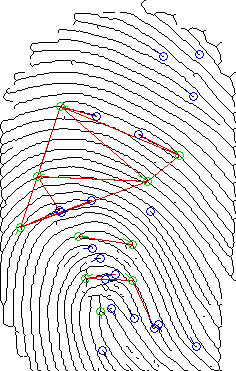
\includegraphics[width=0.9\linewidth]{img/c-final}
		\caption{Graph obtained from the original binary image.}
					\label{fig:concl-c}
	\end{subfigure}%
	\hfill
	\begin{subfigure}{.48\textwidth}
		\centering
		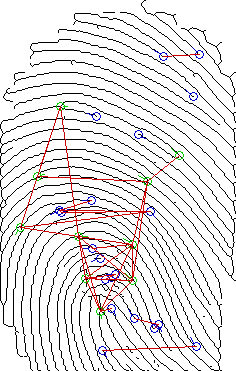
\includegraphics[width=0.86\linewidth]{img/plp-final}
		\caption{Graph obtained from our script.}
			\label{fig:concl-plp}
	\end{subfigure}%
	\caption{Graphs confrontation.}
	\label{fig:concl}
\end{figure}

As future works we plan to:
\begin{enumerate*}[label=\roman*)]
  \item increase the precision of our tool by tuning the equations we described
        or even by introducing more constraints for each type of fingerprint;
  \item automatize the iterative procedure described in
        \cref{sec:graphgen} to permit an easier use of the tool.  This is an
        easy step, which has not been included in this report due to technical
        issue about the installation of \texttt{cplint} in a local machine;
	\item as we have a large set of fingerprints images ($\approx 3\ 000$) we think that 
        exploiting the learning component of \textit{cplint} could bring really promising results.
\end{enumerate*}



%%%%%%%%%%%%%%%%%%%%%%%%%%%%%%%%%%%%%%%%%%%%%%%%%
%%% BIBLIO
%%%%%%%%%%%%%%%%%%%%%%%%%%%%%%%%%%%%%%%%%%%%%%%%%
\bibliography{biblio}
\bibliographystyle{ieeetr}
\end{document}
